%-----------------------------------------------------------------------------------------------------------------------------------------------%
%	The MIT License (MIT)
%
%	Copyright (c) 2015 Jan Küster
%
%	Permission is hereby granted, free of charge, to any person obtaining a copy
%	of this software and associated documentation files (the "Software"), to deal
%	in the Software without restriction, including without limitation the rights
%	to use, copy, modify, merge, publish, distribute, sublicense, and/or sell
%	copies of the Software, and to permit persons to whom the Software is
%	furnished to do so, subject to the following conditions:
%	
%	THE SOFTWARE IS PROVIDED "AS IS", WITHOUT WARRANTY OF ANY KIND, EXPRESS OR
%	IMPLIED, INCLUDING BUT NOT LIMITED TO THE WARRANTIES OF MERCHANTABILITY,
%	FITNESS FOR A PARTICULAR PURPOSE AND NONINFRINGEMENT. IN NO EVENT SHALL THE
%	AUTHORS OR COPYRIGHT HOLDERS BE LIABLE FOR ANY CLAIM, DAMAGES OR OTHER
%	LIABILITY, WHETHER IN AN ACTION OF CONTRACT, TORT OR OTHERWISE, ARISING FROM,
%	OUT OF OR IN CONNECTION WITH THE SOFTWARE OR THE USE OR OTHER DEALINGS IN
%	THE SOFTWARE.
%	
%
%-----------------------------------------------------------------------------------------------------------------------------------------------%


%============================================================================%
%
%	DOCUMENT DEFINITION
%
%============================================================================%

%we use article class because we want to fully customize the page and dont use a cv template
\documentclass[10pt,A4]{article}	


%----------------------------------------------------------------------------------------
%	ENCODING
%----------------------------------------------------------------------------------------

%we use utf8 since we want to build from any machine
\usepackage[utf8]{inputenc}		

%----------------------------------------------------------------------------------------
%	LOGIC
%----------------------------------------------------------------------------------------

% provides \isempty test
\usepackage{xifthen}


%----------------------------------------------------------------------------------------
%	FONT
%----------------------------------------------------------------------------------------

% some tex-live fonts
%\usepackage[defaultsans]{droidsans}
%\usepackage[thin]{comfortaa}
%\usepackage{cmbright}
%\usepackage[default]{raleway}
%\usepackage{fetamont}
\usepackage[default]{gillius}
%\usepackage[light,math]{iwona}
%\usepackage[thin]{roboto} 

% set font default
\renewcommand{\sfdefault}{gillius} 	
\usepackage[T1]{fontenc}

% more font size definitions
\usepackage{moresize}		

%----------------------------------------------------------------------------------------
%	PAGE LAYOUT  DEFINITIONS
%----------------------------------------------------------------------------------------

%debug page outer frames
%\usepackage{showframe}			

%define page styles using geometry
\usepackage[a4paper]{geometry}		

% for example, change the margins to 2 inches all round
\geometry{top=1.5cm, bottom=-.6cm, left=0.8cm, right=0.8cm} 	

%use customized header
\usepackage{fancyhdr}				
\pagestyle{fancy}

%less space between header and content
\setlength{\headheight}{-5pt}		

%customize entries left, center and right
\lhead{}
\chead{ \small{Roman Wilhelm $\cdot$ Team Leader Software Engineer $\cdot$  Paris, France  $\cdot$  \textcolor{sectcol}{\textbf{roman.wlm@gmail.com}}  $\cdot$ +33 672 03 5056}}
\rhead{}

%indentation is zero
\setlength{\parindent}{0mm}

%----------------------------------------------------------------------------------------
%	TABLE /ARRAY/LIST DEFINITIONS
%---------------------------------------------------------------------------------------- 

%for layouting tables
\usepackage{multicol}			
\usepackage{multirow}

%extended aligning of tabular cells
\usepackage{array}

\newcolumntype{x}[1]{%
>{\raggedleft\hspace{0pt}}p{#1}}%

\usepackage{enumitem}


%----------------------------------------------------------------------------------------
%	GRAPHICS DEFINITIONS
%---------------------------------------------------------------------------------------- 

%for header image
\usepackage{graphicx}

%for floating figures
\usepackage{wrapfig}
\usepackage{float}
%\floatstyle{boxed} 
%\restylefloat{figure}

%for drawing graphics		
\usepackage{tikz}				
\usetikzlibrary{shapes, backgrounds, mindmap, trees}


%----------------------------------------------------------------------------------------
%	Color DEFINITIONS
%---------------------------------------------------------------------------------------- 

\usepackage{color}

%accent color
\definecolor{bgcol}{RGB}{0,102,102}

%dark background color / couleur secondaire
\definecolor{sectcol}{RGB}{50,180,150}

%light background / accent color (soulignage)
\definecolor{softcol}{RGB}{4,139,154}


%============================================================================%
%
%
%	DEFINITIONS
%
%
%============================================================================%

%----------------------------------------------------------------------------------------
% 	HEADER
%----------------------------------------------------------------------------------------

% remove top header line
\renewcommand{\headrulewidth}{0pt} 

%remove botttom header line
\renewcommand{\footrulewidth}{0pt}	  	

%remove pagenum
\renewcommand{\thepage}{}	

%remove section num		
\renewcommand{\thesection}{}			

%----------------------------------------------------------------------------------------
% 	ARROW GRAPHICS in Tikz
%----------------------------------------------------------------------------------------

% a six pointed arrow poiting to the left
\newcommand{\tzlarrow}{(0,0) -- (0.2,0) -- (0.3,0.2) -- (0.2,0.4) -- (0,0.4) -- (0.1,0.2) -- cycle;}	

% include the left arrow into a tikz picture
% param1: fill color
%
\newcommand{\larrow}[1]
{\begin{tikzpicture}[scale=0.58]
	 \filldraw[fill=#1!100,draw=#1!100!black]  \tzlarrow
 \end{tikzpicture}
}

% a six pointed arrow poiting to the right
\newcommand{\tzrarrow}{ (0,0.2) -- (0.1,0) -- (0.3,0) -- (0.2,0.2) -- (0.3,0.4) -- (0.1,0.4) -- cycle;}

% include the right arrow into a tikz picture
% param1: fill color
%
\newcommand{\rarrow}
{
\begin{tikzpicture}[scale=0.7]
	\filldraw[fill=sectcol!100,draw=sectcol!100!black] \tzrarrow
 \end{tikzpicture}
}

%----------------------------------------------------------------------------------------
%	custom sections
%----------------------------------------------------------------------------------------

% create a coloured box with arrow and title as cv section headline
% param 1: section title
%
\newcommand{\cvsection}[1]
{
\colorbox{bgcol}{\makebox[1\linewidth][l]{
	\larrow{sectcol} \hspace{-8pt} \larrow{sectcol} \hspace{-8pt} \larrow{sectcol} \textcolor{white}{\textbf{#1}}\hspace{4pt}
}}\\
}

%create a coloured arrow with title as cv meta section section
% param 1: meta section title
%
\newcommand{\metasection}[2]{
	\begin{tabular*}{1\linewidth}{p{0.18\linewidth} p{0.76\linewidth}}
		\larrow{bgcol}\normalsize{\textbf{\textcolor{sectcol}{#1}}}&#2\\
	\end{tabular*}
}

%----------------------------------------------------------------------------------------
%	 CV EVENT
%----------------------------------------------------------------------------------------

% creates a stretched box as cv entry headline followed by two paragraphs about 
% the work you did
% param 1:	event time i.e. 2014 or 2011-2014 etc.
% param 2:	Role 
% param 3:	institution 
% param 4+:	Details
%
\newcommand{\cveventfour}[7] {
\begin{flushleft}
\textcolor{sectcol}{#1 - #3}\\
\textbf{#2}\\[-7pt]
\textcolor{softcol}{\hrule}
\vspace{\spread}
\begin{tabular*}{1\linewidth}{p{0.001\linewidth} p{0.9\linewidth}}
	\larrow{bgcol} & #4 \\[2pt]
	\larrow{bgcol} & #5 \\[2pt]
	\larrow{bgcol} & #6 \\[2pt]
	\larrow{bgcol} & #7 \\[\spread]
\end{tabular*}
\end{flushleft}
%\textcolor{softcol}{\hrule}
}

\newcommand{\cveventthree}[6] {
\begin{flushleft}
\textcolor{sectcol}{#1 - #3}\\
\textbf{#2}\\[-7pt]
\textcolor{softcol}{\hrule}
\vspace{\spread}
\begin{tabular*}{1\linewidth}{p{0.001\linewidth} p{0.9\linewidth}}
	\larrow{bgcol} & #4 \\[2pt]
	\larrow{bgcol} & #5 \\[2pt]
	\larrow{bgcol} & #6 \\[\spread]
\end{tabular*}
\end{flushleft}
%\textcolor{softcol}{\hrule}
}

\newcommand{\cveventtwo}[5] {
\begin{flushleft}
\textcolor{sectcol}{#1 - #3}\\
\textbf{#2}\\[-7pt]
\textcolor{softcol}{\hrule}
\vspace{\spread}
\begin{tabular*}{1\linewidth}{p{0.001\linewidth} p{0.9\linewidth}}
	\larrow{bgcol} & #4 \\[2pt]
	\larrow{bgcol} & #5 \\[\spread]
\end{tabular*}
\end{flushleft}
%\textcolor{softcol}{\hrule}
}

\newcommand{\cveventone}[4] {
\begin{flushleft}
\textcolor{sectcol}{#1 - #3}\\
\textbf{#2}\\[-7pt]
\textcolor{softcol}{\hrule}
\vspace{\spread}
\begin{tabular*}{1\linewidth}{p{0.001\linewidth} p{0.9\linewidth}}
	\larrow{bgcol} & #4 \\[\spread]
\end{tabular*}
\end{flushleft}
%\textcolor{softcol}{\hrule}
}

% Customs For skill part
\newcommand{\skidev}[9] {
\begin{flushleft}
\textbf{#1}\\[-7pt]
\vspace{\spread}
\begin{tabular*}{1\linewidth}{p{0.001\linewidth} p{0.9\linewidth}}
	\larrow{bgcol} & \textcolor{sectcol}{#2} #3 \\[2pt]
	\larrow{bgcol} & \textcolor{sectcol}{#4} #5 \\[2pt]
	\larrow{bgcol} & \textcolor{sectcol}{#6} #7 \\[2pt]
	\larrow{bgcol} & \textcolor{sectcol}{#8} #9\\[\spread]
\end{tabular*}
\end{flushleft}
}

\newcommand{\skilang}[7] {
\begin{flushleft}
\textbf{#1}\\[-7pt]
\vspace{\spread}
\begin{tabular*}{1\linewidth}{p{0.001\linewidth} p{0.9\linewidth}}
	\larrow{bgcol} & \textcolor{sectcol}{#2} #3 \\[2pt]
	\larrow{bgcol} & \textcolor{sectcol}{#4} #5 \\[2pt]
	\larrow{bgcol} & \textcolor{sectcol}{#6} #7\\[\spread]
\end{tabular*}
\end{flushleft}
}

\newcommand{\skienv}[5] {
\begin{flushleft}
\textbf{#1}\\[-7pt]
\vspace{\spread}
\begin{tabular*}{1\linewidth}{p{0.001\linewidth} p{0.9\linewidth}}
	\larrow{bgcol} & \textcolor{sectcol}{#2} #3 \\[2pt]
	\larrow{bgcol} & \textcolor{sectcol}{#4} #5\\[\spread]
\end{tabular*}
\end{flushleft}
}

% creates a stretched box as 
\newcommand{\cveventmeta}[4] {
	\mbox{\mystrut \hspace{87pt}\textit{#1}}\\
	#2
}

%----------------------------------------------------------------------------------------
% CUSTOM STRUT FOR EMPTY BOXES
%----------------------------------------- -----------------------------------------------
\newcommand{\mystrut}{\rule[-.3\baselineskip]{0pt}{\baselineskip}}

%----------------------------------------------------------------------------------------
% SPREAD
%----------------------------------------------------------------------------------------
\newcommand{\spread}{7pt}

%============================================================================%
%
%
%
%	DOCUMENT CONTENT
%
%
%
%============================================================================%
\begin{document}

%use our custom fancy header definitions
\pagestyle{fancy}

\begin{minipage}[t]{0.485\textwidth}

\vspace{\spread}

%---------------------------------------------------------------------------------------
%	TITLE HEADLINE
%----------------------------------------------------------------------------------------

\hspace{0.0\linewidth}\colorbox{bgcol}
{
	\makebox[1.00\linewidth][c]{
		\fontsize{24pt}{0pt}{\textcolor{white}{\textsc{Roman}}} 
		{\textcolor{white}{\textsc{Wilhelm}} } }}
\bigbreak
\bigbreak
%\hspace{-0.25\linewidth}\colorbox{bgcol}{\makebox[1.25\linewidth][c]{\HUGE{\textcolor{white}{\textsc{Roman}} } \textcolor{sectcol}{\rule[-1mm]{1mm}{0.9cm}} \HUGE{\textcolor{white}{\textsc{Wilhelm}} } }}

%----------------------------------------------------------------------------------------
%	HEADER IMAGE
%----------------------------------------------------------------------------------------

\hspace{5.87cm}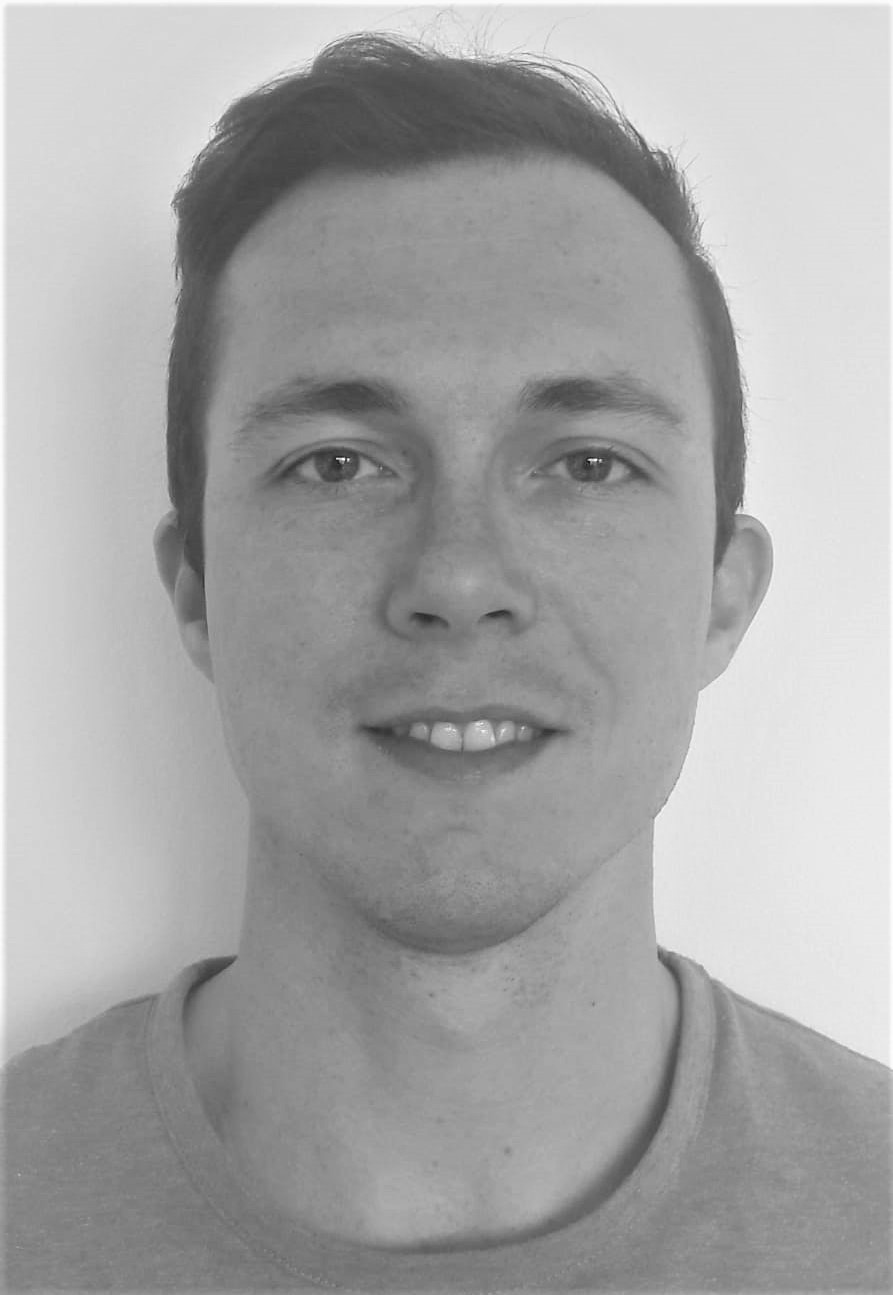
\includegraphics[scale=0.13]{img/PhotoProfil.jpeg} %use full size

%---------------------------------------------------------------------------------------
%	WORD CLOUD IMG
%----------------------------------------------------------------------------------------
\vspace{-110pt}
%\hspace{0.59\linewidth}
\hspace{0.00cm}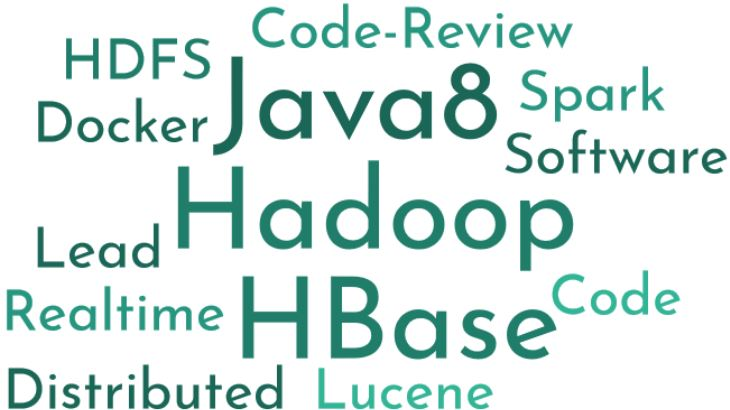
\includegraphics[scale=0.3]{img/Nuage.jpg}
\normalsize
\vspace{20pt}
\vspace{\spread}

\end{minipage} 
\hfill
\begin{minipage}[t]{0.485\textwidth}
%---------------------------------------------------------------------------------------
%	SUMMARY (optional)
%----------------------------------------------------------------------------------------
\vspace{\spread}

\cvsection{Summary}\\
I am Software Engineer specialized on distributed environements. 
\smallbreak
I worked during 6 years into a startup company with various responsabilities from design and implements low layers of application, implements business cases up to team management. 
\smallbreak
We recently raised funds, our product is now production-ready and a first set of client is using it for their regulations report purposes. 
\smallbreak Nowaday, I would like to discover new horizons with new challenges.\\[-2pt]
\textcolor{softcol}{\hrule}

\end{minipage}

\begin{minipage}[t]{0.485\textwidth}

\vspace{\spread}

%---------------------------------------------------------------------------------------
%	META SECTION
%----------------------------------------------------------------------------------------
\metasection{Status}{Team Leader, Big Data Back-End Engineer}
%\metasection{Fields:}{Team Management, Software Development} 
\metasection{Loves}{Music, Art and Design, Craft and Renovate}
\end{minipage}
\hfill
\begin{minipage}[t]{0.485\textwidth}

\vspace{5pt}

\metasection{Skills}{Java 8, HBase, HDFS, Zookeeper, Lucene}
	%, Linux, Git, IntelliJ}
\metasection{Friendly}{Docker, Yarn, Spark, Kafka, Python, Bash}
%\metasection{Loves:}{Music, Football, Art and Design, DIY}

\end{minipage}
\hfill
\begin{minipage}[t]{0.485\textwidth}
\vspace{\spread}

%---------------------------------------------------------------------------------------
%	EDUCATION SECTION
%--------------------------------------------------------------------------------------

\cvsection{Education}
\cveventfour{2009 / 2012}{Egineering Graduate}{Polytech' Montpellier}
	{Engineering Degree Computer Science and Management}
	{Software engineering and project management}	
	{Oriented Object / Functional Programming, Networks} 
	{Statistics, RO, Management}   

\cveventtwo{2011 / 2012}{Master - Economic Information System for Enterprise}{Economic University of Montpellier}
	{Basics of Datamining and TextMining}
	{Supervised and Unsupervised Machine Learning Algorithms}
 
\cveventthree{2007 / 2009}{DUT Computer Science and Management}{IUT - Montpelier Institute of Technology}
	{Oriented Object Programation}
	{Modeling methodologies Merise / UML}	
	{Accountancy, HMI }


%---------------------------------------------------------------------------------------
%	SKILLS SECTION
%--------------------------------------------------------------------------------------

\cvsection{Detailed Skills}
\skilang{Languages}
	{Expert :}{Java JDK 8, Multithreading}
	{Ready :}{Bash, SQL}	 
	{Beginner :}{Python, Scala}   
	
\skidev{Development}
	{Methodologies :}{ Scrum, Test Driven Development}
	{Dev tools :}{ Git, Jira, Maven, TeamCity}
	{Profiling :}{ Yourkit, JStack, JVisualVM}
	{Techno :}{ Hadoop, HDFS, ZK, HBase, Lucene, Spark, Kafka, Protobuf}
	
\skienv{Environment}
	{Container :}{ Docker }
	{Operating System :}{ Ubuntu, CentOs}
	
%---------------------------------------------------------------------------------------
%	CHANGE TO RIGHT SIDE PART 
%----------------------------------------------------------------------------------------
\end{minipage}
\hfill
\begin{minipage}[t]{0.485\textwidth}
\vspace{\spread}

%---------------------------------------------------------------------------------------
%	EXPERIENCE
%----------------------------------------------------------------------------------------
\cvsection{Experience}
\cveventfour{2016 / 2019}{Team Leader}{Scaled Risk}
	{Stand-up meeting animation and team planning}
	{Code review sessions, Setting up code quality}  
	{Lead a team of 4 peoples}
	{Recruitment sessions}

%
\cveventfour{2013 / 2016}{Solution Engineer}{Scaled Risk}
	{Implements oriented-object metamodel over HBase}
	{Distributed indexation engine with Lucene}
	{Distributed consensus with Zookeeper}
	{Multi-temporal storage and indexation}
%
\cveventtwo{2012 / 6 months}{Internship Datamining}{International retail banking - BHFM/Société Générale - Paris, La Defense}
	{Various missions around churn phenomenon study, Definining customers profiles and attrition behaviour}
	{MCA, Decision trees, Descriptives statistics}

%
\cveventtwo{2011 / 3 months}{Internship R\&D in Computer Lab}{Concordia University - Montreal, Canada}
	{As part of a team responsible to implement a data visualisation system on top of a an innovative distributed data warehouse system}
	{OLAP System, Java, Smart GWT}

%
\cveventone{2009 / 3 months}{Internship in Computer Lab}{University of Central Lancashire - Preston, UK}
	{ChiCI Lab, Child computer Interaction. Specification and implementation of a ludic platform to socialize children with difficults. Interaction with Wiimote}
%	{Java, Swing, Connect Wiimote by Bluetooth and moteJ} 

\end{minipage}

%-------------------------------------------------------------------------------------------------
%	ARTIFICIAL FOOTER (fancy footer cannot exceed linewidth) 
%--------------------------------------------------------------------------------------------------

\null
\vspace*{\fill}
\hspace{-0.25\linewidth}\colorbox{bgcol}{\makebox[1.5\linewidth][c]{\mystrut \small \textcolor{white}{www.linkedin.com/in/romanwilhelm} $\cdot$ \textcolor{white}{github.com/romanwlm}}}


%============================================================================%
%
%
%
%	DOCUMENT END
%
%
%
%============================================================================%
\end{document}
